%%%%%%%%%%%%%%%%%%%%%%%%%%%%%%%%%%%%%%%%
%
% Important note:
% Chapter heading images should have a 2:1 width:height ratio,
% e.g. 920px width and 460px height.
%
%%%%%%%%%%%%%%%%%%%%%%%%%%%%%%%%%%%%%%%%%

%----------------------------------------------------------------------------------------
%    PACKAGES AND OTHER DOCUMENT CONFIGURATIONS
%----------------------------------------------------------------------------------------

\documentclass[11pt,fleqn]{book} % Default font size and left-justified equations

\usepackage[top=3cm,bottom=3cm,left=3.2cm,right=3.2cm,headsep=10pt,letterpaper]{geometry} % Page margins

\usepackage{xcolor} % Required for specifying colors by name
\definecolor{ocre}{RGB}{52,177,201} % Define the orange color used for highlighting throughout

% Font Settings
\usepackage{avant} % Use the Avantgarde font for headings
%\usepackage{times} % Use the Times font for headings
\usepackage{mathptmx} % Use the Adobe Times Roman as the default text font together with math symbols from the Sym­bol, Chancery and Com­puter Modern fonts

\usepackage{microtype} % Slightly tweak font spacing for aesthetics
\usepackage[utf8]{inputenc} % Required for including letters with accents
\usepackage[T1]{fontenc} % Use 8-bit encoding that has 256 glyphs

% Bibliography
\usepackage[style=alphabetic,sorting=nyt,sortcites=true,autopunct=true,babel=hyphen,hyperref=true,abbreviate=false,backref=true,backend=biber]{biblatex}
\addbibresource{bibliography.bib} % BibTeX bibliography file
\defbibheading{bibempty}{}

%----------------------------------------------------------------------------------------
%	VARIOUS REQUIRED PACKAGES
%----------------------------------------------------------------------------------------

\usepackage{titlesec} % Allows customization of titles

\usepackage{graphicx} % Required for including pictures
\graphicspath{{Pictures/}} % Specifies the directory where pictures are stored

\usepackage{lipsum} % Inserts dummy text

\usepackage{tikz} % Required for drawing custom shapes

\usepackage[english]{babel} % English language/hyphenation

\usepackage{enumitem} % Customize lists
\setlist{nolistsep} % Reduce spacing between bullet points and numbered lists

\usepackage{booktabs} % Required for nicer horizontal rules in tables

\usepackage{eso-pic} % Required for specifying an image background in the title page

%----------------------------------------------------------------------------------------
%	MAIN TABLE OF CONTENTS
%----------------------------------------------------------------------------------------

\usepackage{titletoc} % Required for manipulating the table of contents

\contentsmargin{0cm} % Removes the default margin
% Chapter text styling
\titlecontents{chapter}[1.25cm] % Indentation
{\addvspace{15pt}\large\sffamily\bfseries} % Spacing and font options for chapters
{\color{ocre!60}\contentslabel[\Large\thecontentslabel]{1.25cm}\color{ocre}} % Chapter number
{}  
{\color{ocre!60}\normalsize\sffamily\bfseries\;\titlerule*[.5pc]{.}\;\thecontentspage} % Page number
% Section text styling
\titlecontents{section}[1.25cm] % Indentation
{\addvspace{5pt}\sffamily\bfseries} % Spacing and font options for sections
{\contentslabel[\thecontentslabel]{1.25cm}} % Section number
{}
{\sffamily\hfill\color{black}\thecontentspage} % Page number
[]
% Subsection text styling
\titlecontents{subsection}[1.25cm] % Indentation
{\addvspace{1pt}\sffamily\small} % Spacing and font options for subsections
{\contentslabel[\thecontentslabel]{1.25cm}} % Subsection number
{}
{\sffamily\;\titlerule*[.5pc]{.}\;\thecontentspage} % Page number
[] 

%----------------------------------------------------------------------------------------
%	MINI TABLE OF CONTENTS IN CHAPTER HEADS
%----------------------------------------------------------------------------------------

% Section text styling
\titlecontents{lsection}[0em] % Indendating
{\footnotesize\sffamily} % Font settings
{}
{}
{}

% Subsection text styling
\titlecontents{lsubsection}[.5em] % Indentation
{\normalfont\footnotesize\sffamily} % Font settings
{}
{}
{}
 
%----------------------------------------------------------------------------------------
%	PAGE HEADERS
%----------------------------------------------------------------------------------------

\usepackage{fancyhdr} % Required for header and footer configuration

\pagestyle{fancy}
\renewcommand{\chaptermark}[1]{\markboth{\sffamily\normalsize\bfseries\chaptername\ \thechapter.\ #1}{}} % Chapter text font settings
\renewcommand{\sectionmark}[1]{\markright{\sffamily\normalsize\thesection\hspace{5pt}#1}{}} % Section text font settings
\fancyhf{} \fancyhead[LE,RO]{\sffamily\normalsize\thepage} % Font setting for the page number in the header
\fancyhead[LO]{\rightmark} % Print the nearest section name on the left side of odd pages
\fancyhead[RE]{\leftmark} % Print the current chapter name on the right side of even pages
\renewcommand{\headrulewidth}{0.5pt} % Width of the rule under the header
\addtolength{\headheight}{2.5pt} % Increase the spacing around the header slightly
\renewcommand{\footrulewidth}{0pt} % Removes the rule in the footer
\fancypagestyle{plain}{\fancyhead{}\renewcommand{\headrulewidth}{0pt}} % Style for when a plain pagestyle is specified

% Removes the header from odd empty pages at the end of chapters
\makeatletter
\renewcommand{\cleardoublepage}{
\clearpage\ifodd\c@page\else
\hbox{}
\vspace*{\fill}
\thispagestyle{empty}
\newpage
\fi}

%----------------------------------------------------------------------------------------
%	THEOREM STYLES
%----------------------------------------------------------------------------------------

\usepackage{amsmath,amsfonts,amssymb,amsthm} % For math equations, theorems, symbols, etc

\newcommand{\intoo}[2]{\mathopen{]}#1\,;#2\mathclose{[}}
\newcommand{\ud}{\mathop{\mathrm{{}d}}\mathopen{}}
\newcommand{\intff}[2]{\mathopen{[}#1\,;#2\mathclose{]}}
\newtheorem{notation}{Notation}[chapter]

%%%%%%%%%%%%%%%%%%%%%%%%%%%%%%%%%%%%%%%%%%%%%%%%%%%%%%%%%%%%%%%%%%%%%%%%%%%
%%%%%%%%%%%%%%%%%%%% dedicated to boxed/framed environements %%%%%%%%%%%%%%
%%%%%%%%%%%%%%%%%%%%%%%%%%%%%%%%%%%%%%%%%%%%%%%%%%%%%%%%%%%%%%%%%%%%%%%%%%%
\newtheoremstyle{ocrenumbox}% % Theorem style name
{0pt}% Space above
{0pt}% Space below
{\normalfont}% % Body font
{}% Indent amount
{\small\bf\sffamily\color{ocre}}% % Theorem head font
{\;}% Punctuation after theorem head
{0.25em}% Space after theorem head
{\small\sffamily\color{ocre}\thmname{#1}\nobreakspace\thmnumber{\@ifnotempty{#1}{}\@upn{#2}}% Theorem text (e.g. Theorem 2.1)
\thmnote{\nobreakspace\the\thm@notefont\sffamily\bfseries\color{black}---\nobreakspace#3.}} % Optional theorem note
\renewcommand{\qedsymbol}{$\blacksquare$}% Optional qed square

\newtheoremstyle{blacknumex}% Theorem style name
{5pt}% Space above
{5pt}% Space below
{\normalfont}% Body font
{} % Indent amount
{\small\bf\sffamily}% Theorem head font
{\;}% Punctuation after theorem head
{0.25em}% Space after theorem head
{\small\sffamily{\tiny\ensuremath{\blacksquare}}\nobreakspace\thmname{#1}\nobreakspace\thmnumber{\@ifnotempty{#1}{}\@upn{#2}}% Theorem text (e.g. Theorem 2.1)
\thmnote{\nobreakspace\the\thm@notefont\sffamily\bfseries---\nobreakspace#3.}}% Optional theorem note

\newtheoremstyle{blacknumbox} % Theorem style name
{0pt}% Space above
{0pt}% Space below
{\normalfont}% Body font
{}% Indent amount
{\small\bf\sffamily}% Theorem head font
{\;}% Punctuation after theorem head
{0.25em}% Space after theorem head
{\small\sffamily\thmname{#1}\nobreakspace\thmnumber{\@ifnotempty{#1}{}\@upn{#2}}% Theorem text (e.g. Theorem 2.1)
\thmnote{\nobreakspace\the\thm@notefont\sffamily\bfseries---\nobreakspace#3.}}% Optional theorem note

%%%%%%%%%%%%%%%%%%%%%%%%%%%%%%%%%%%%%%%%%%%%%%%%%%%%%%%%%%%%%%%%%%%%%%%%%%%
%%%%%%%%%%%%% dedicated to non-boxed/non-framed environements %%%%%%%%%%%%%
%%%%%%%%%%%%%%%%%%%%%%%%%%%%%%%%%%%%%%%%%%%%%%%%%%%%%%%%%%%%%%%%%%%%%%%%%%%
\newtheoremstyle{ocrenum}% % Theorem style name
{5pt}% Space above
{5pt}% Space below
{\normalfont}% % Body font
{}% Indent amount
{\small\bf\sffamily\color{ocre}}% % Theorem head font
{\;}% Punctuation after theorem head
{0.25em}% Space after theorem head
{\small\sffamily\color{ocre}\thmname{#1}\nobreakspace\thmnumber{\@ifnotempty{#1}{}\@upn{#2}}% Theorem text (e.g. Theorem 2.1)
\thmnote{\nobreakspace\the\thm@notefont\sffamily\bfseries\color{black}---\nobreakspace#3.}} % Optional theorem note
\renewcommand{\qedsymbol}{$\blacksquare$}% Optional qed square
\makeatother

% Defines the theorem text style for each type of theorem to one of the three styles above
\newcounter{dummy} 
\numberwithin{dummy}{section}
\theoremstyle{ocrenumbox}
\newtheorem{theoremeT}[dummy]{Theorem}
\newtheorem{problem}{Problem}[chapter]
\newtheorem{exerciseT}{Exercise}[chapter]
\theoremstyle{blacknumex}
\newtheorem{exampleT}{Example}[chapter]
\theoremstyle{blacknumbox}
\newtheorem{vocabulary}{Vocabulary}[chapter]
\newtheorem{definitionT}{Definition}[section]
\newtheorem{corollaryT}[dummy]{Corollary}
\theoremstyle{ocrenum}
\newtheorem{proposition}[dummy]{Proposition}

%----------------------------------------------------------------------------------------
%	DEFINITION OF COLORED BOXES
%----------------------------------------------------------------------------------------

\RequirePackage[framemethod=default]{mdframed} % Required for creating the theorem, definition, exercise and corollary boxes

% Theorem box
\newmdenv[skipabove=7pt,
skipbelow=7pt,
backgroundcolor=black!5,
linecolor=ocre,
innerleftmargin=5pt,
innerrightmargin=5pt,
innertopmargin=5pt,
leftmargin=0cm,
rightmargin=0cm,
innerbottommargin=5pt]{tBox}

% Exercise box	  
\newmdenv[skipabove=7pt,
skipbelow=7pt,
rightline=false,
leftline=true,
topline=false,
bottomline=false,
backgroundcolor=ocre!10,
linecolor=ocre,
innerleftmargin=5pt,
innerrightmargin=5pt,
innertopmargin=5pt,
innerbottommargin=5pt,
leftmargin=0cm,
rightmargin=0cm,
linewidth=4pt]{eBox}	

% Definition box
\newmdenv[skipabove=7pt,
skipbelow=7pt,
rightline=false,
leftline=true,
topline=false,
bottomline=false,
linecolor=ocre,
innerleftmargin=5pt,
innerrightmargin=5pt,
innertopmargin=0pt,
leftmargin=0cm,
rightmargin=0cm,
linewidth=4pt,
innerbottommargin=0pt]{dBox}	

% Corollary box
\newmdenv[skipabove=7pt,
skipbelow=7pt,
rightline=false,
leftline=true,
topline=false,
bottomline=false,
linecolor=gray,
backgroundcolor=black!5,
innerleftmargin=5pt,
innerrightmargin=5pt,
innertopmargin=5pt,
leftmargin=0cm,
rightmargin=0cm,
linewidth=4pt,
innerbottommargin=5pt]{cBox}

% Creates an environment for each type of theorem and assigns it a theorem text style from the "Theorem Styles" section above and a colored box from above
\newenvironment{theorem}{\begin{tBox}\begin{theoremeT}}{\end{theoremeT}\end{tBox}}
\newenvironment{exercise}{\begin{eBox}\begin{exerciseT}}{\hfill{\color{ocre}\tiny\ensuremath{\blacksquare}}\end{exerciseT}\end{eBox}}				  
\newenvironment{definition}{\begin{dBox}\begin{definitionT}}{\end{definitionT}\end{dBox}}	
\newenvironment{example}{\begin{exampleT}}{\hfill{\tiny\ensuremath{\blacksquare}}\end{exampleT}}		
\newenvironment{corollary}{\begin{cBox}\begin{corollaryT}}{\end{corollaryT}\end{cBox}}	

%----------------------------------------------------------------------------------------
%	REMARK ENVIRONMENT
%----------------------------------------------------------------------------------------

\newenvironment{remark}{\par\vspace{10pt}\small % Vertical white space above the remark and smaller font size
\begin{list}{}{
\leftmargin=35pt % Indentation on the left
\rightmargin=25pt}\item\ignorespaces % Indentation on the right
\makebox[-2.5pt]{\begin{tikzpicture}[overlay]
\node[draw=ocre!60,line width=1pt,circle,fill=ocre!25,font=\sffamily\bfseries,inner sep=2pt,outer sep=0pt] at (-15pt,0pt){\textcolor{ocre}{R}};\end{tikzpicture}} % Orange R in a circle
\advance\baselineskip -1pt}{\end{list}\vskip5pt} % Tighter line spacing and white space after remark

%----------------------------------------------------------------------------------------
%	SECTION NUMBERING IN THE MARGIN
%----------------------------------------------------------------------------------------

\makeatletter
\renewcommand{\@seccntformat}[1]{\llap{\textcolor{ocre}{\csname the#1\endcsname}\hspace{1em}}}                    
\renewcommand{\section}{\@startsection{section}{1}{\z@}
{-4ex \@plus -1ex \@minus -.4ex}
{1ex \@plus.2ex }
{\normalfont\large\sffamily\bfseries}}
\renewcommand{\subsection}{\@startsection {subsection}{2}{\z@}
{-3ex \@plus -0.1ex \@minus -.4ex}
{0.5ex \@plus.2ex }
{\normalfont\sffamily\bfseries}}
\renewcommand{\subsubsection}{\@startsection {subsubsection}{3}{\z@}
{-2ex \@plus -0.1ex \@minus -.2ex}
{.2ex \@plus.2ex }
{\normalfont\small\sffamily\bfseries}}                        
\renewcommand\paragraph{\@startsection{paragraph}{4}{\z@}
{-2ex \@plus-.2ex \@minus .2ex}
{.1ex}
{\normalfont\small\sffamily\bfseries}}

%----------------------------------------------------------------------------------------
%	HYPERLINKS IN THE DOCUMENTS
%----------------------------------------------------------------------------------------

% For an unclear reason, the package should be loaded now and not later
\usepackage{hyperref}
\hypersetup{hidelinks,backref=true,pagebackref=true,hyperindex=true,colorlinks=false,breaklinks=true,urlcolor= ocre,bookmarks=true,bookmarksopen=false,pdftitle={Title},pdfauthor={Author}}

%----------------------------------------------------------------------------------------
%	CHAPTER HEADINGS
%----------------------------------------------------------------------------------------

% The set-up below should be (sadly) manually adapted to the overall margin page septup controlled by the geometry package loaded in the main.tex document. It is possible to implement below the dimensions used in the goemetry package (top,bottom,left,right)... TO BE DONE

\newcommand{\thechapterimage}{}
\newcommand{\chapterimage}[1]{\renewcommand{\thechapterimage}{#1}}

% Numbered chapters with mini tableofcontents
\def\thechapter{\arabic{chapter}}
\def\@makechapterhead#1{
\thispagestyle{empty}
{\centering \normalfont\sffamily
\ifnum \c@secnumdepth >\m@ne
\if@mainmatter
\startcontents
\begin{tikzpicture}[remember picture,overlay]
\node at (current page.north west)
{\begin{tikzpicture}[remember picture,overlay]
\node[anchor=north west,inner sep=0pt] at (0,0) {\includegraphics[width=\paperwidth]{\thechapterimage}};
%%%%%%%%%%%%%%%%%%%%%%%%%%%%%%%%%%%%%%%%%%%%%%%%%%%%%%%%%%%%%%%%%%%%%%%%%%%%%%%%%%%%%
% Commenting the 3 lines below removes the small contents box in the chapter heading
%\fill[color=ocre!10!white,opacity=.6] (1cm,0) rectangle (8cm,-7cm);
%\node[anchor=north west] at (1.1cm,.35cm) {\parbox[t][8cm][t]{6.5cm}{\huge\bfseries\flushleft \printcontents{l}{1}{\setcounter{tocdepth}{2}}}};
\draw[anchor=west] (5cm,-9cm) node [rounded corners=20pt,fill=ocre!10!white,text opacity=1,draw=ocre,draw opacity=1,line width=1.5pt,fill opacity=.6,inner sep=12pt]{\huge\sffamily\bfseries\textcolor{black}{\thechapter. #1\strut\makebox[22cm]{}}};
%%%%%%%%%%%%%%%%%%%%%%%%%%%%%%%%%%%%%%%%%%%%%%%%%%%%%%%%%%%%%%%%%%%%%%%%%%%%%%%%%%%%%
\end{tikzpicture}};
\end{tikzpicture}}
\par\vspace*{230\p@}
\fi
\fi}

% Unnumbered chapters without mini tableofcontents (could be added though) 
\def\@makeschapterhead#1{
\thispagestyle{empty}
{\centering \normalfont\sffamily
\ifnum \c@secnumdepth >\m@ne
\if@mainmatter
\begin{tikzpicture}[remember picture,overlay]
\node at (current page.north west)
{\begin{tikzpicture}[remember picture,overlay]
\node[anchor=north west,inner sep=0pt] at (0,0) {\includegraphics[width=\paperwidth]{\thechapterimage}};
\draw[anchor=west] (5cm,-9cm) node [rounded corners=20pt,fill=ocre!10!white,fill opacity=.6,inner sep=12pt,text opacity=1,draw=ocre,draw opacity=1,line width=1.5pt]{\huge\sffamily\bfseries\textcolor{black}{#1\strut\makebox[22cm]{}}};
\end{tikzpicture}};
\end{tikzpicture}}
\par\vspace*{230\p@}
\fi
\fi
}
\makeatother % Insert the commands.tex file which contains the majority of the structure behind the template

\begin{document}
\setlength{\parskip}{2ex}
%----------------------------------------------------------------------------------------
%    TITLE PAGE
%----------------------------------------------------------------------------------------

\begingroup
\thispagestyle{empty}
\AddToShipoutPicture*{\put(0,0){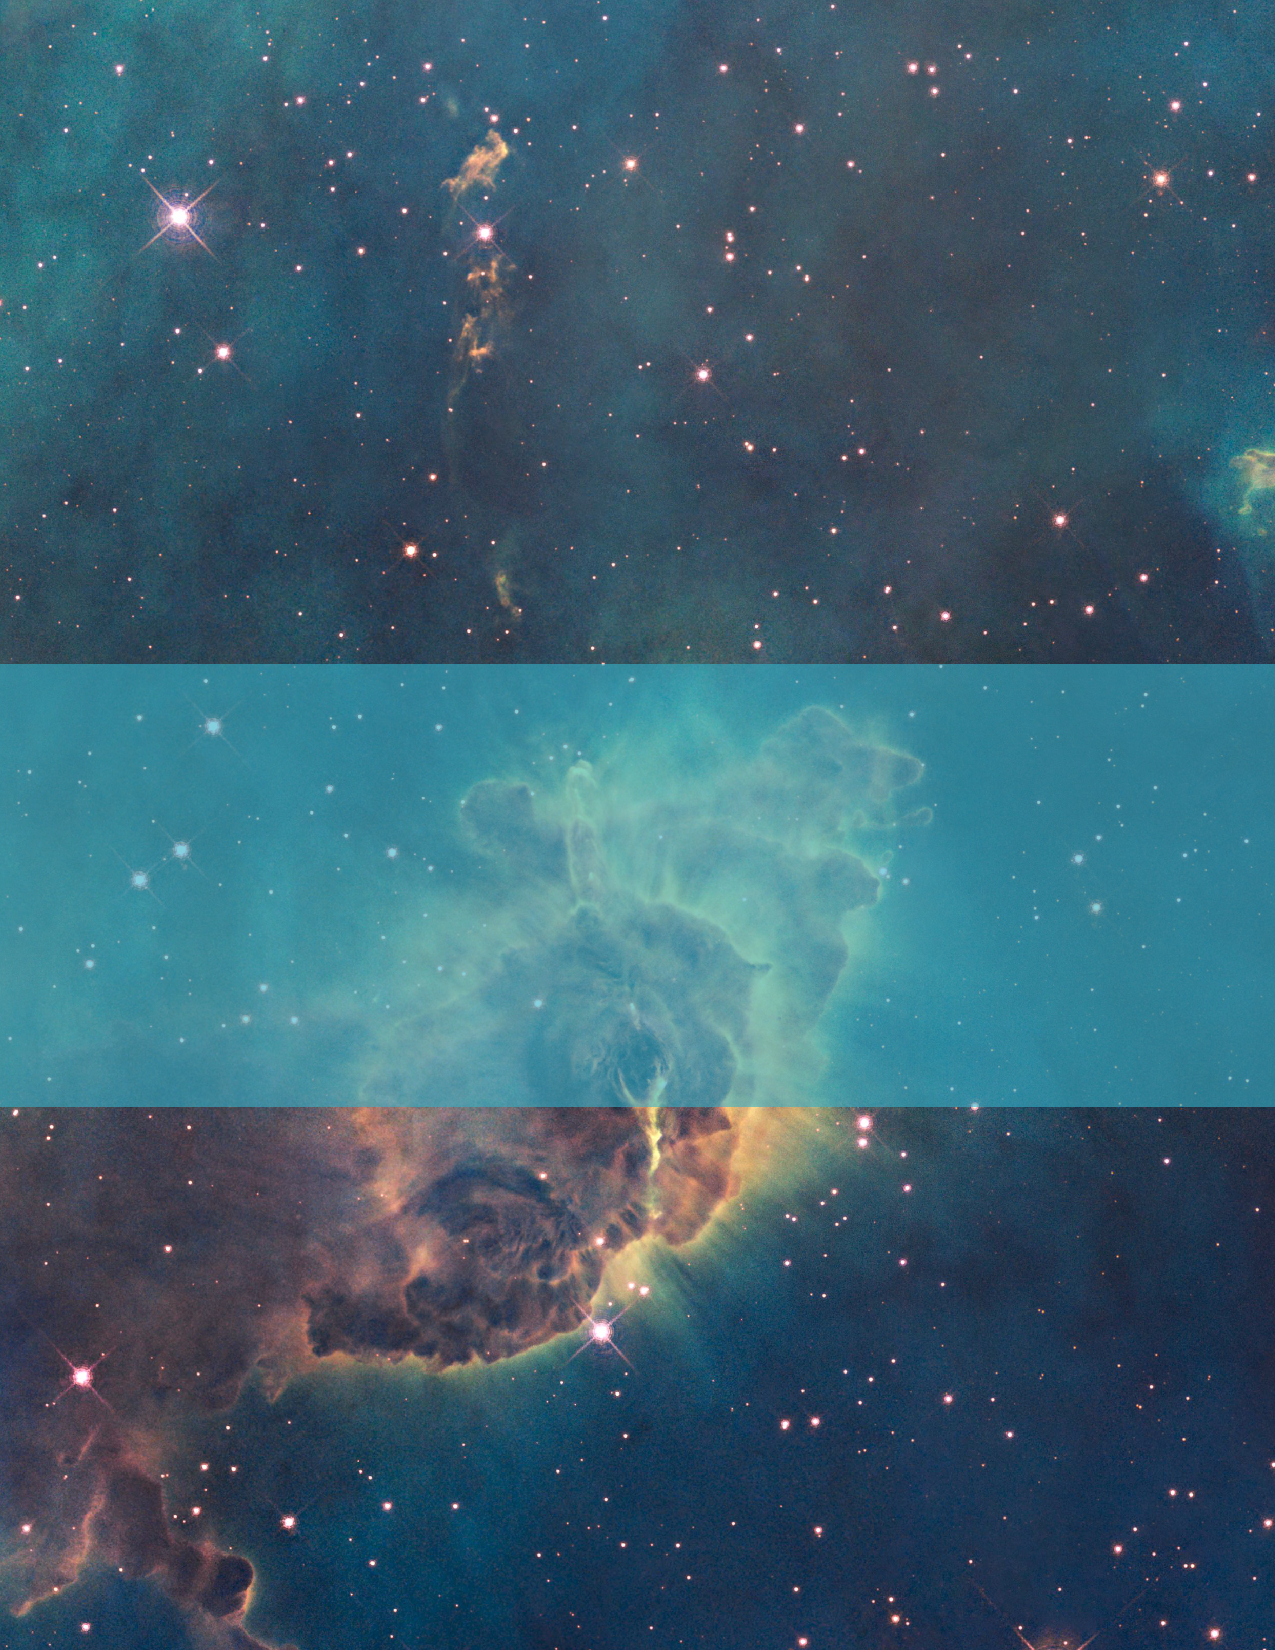
\includegraphics[scale=1.25]{media/esahubble.png}}} % Image background
\centering
\vspace*{5cm}
\par\normalfont\fontsize{35}{35}\sffamily\selectfont
\textbf{Modelling and Simulation on SpatialOS}\\
{\LARGE Exploring the ScienceSDK}\par % Book title
\vspace*{1cm}

\includegraphics[width=0.5\textwidth]{media/Improbable_full-black.eps}
\par % Author name
\vspace{30mm}
\centering
\color{red} {\LARGE \textbf{WORK IN PROGRESS - PRE-RELEASE}}\color{black}
\endgroup

%----------------------------------------------------------------------------------------
%    COPYRIGHT PAGE
%----------------------------------------------------------------------------------------

\newpage
~\vfill
\thispagestyle{empty}

%\noindent Copyright \copyright\ 2017 Improbable\\ % Copyright notice

\noindent \textsc{Improbable}\\

\noindent \textsc{github.com/improbable-io/ScienceOS}\\ % URL

\noindent 
For more information contact daveculley@improbable.io\\ %

\noindent \textit{First release, 2017} % Printing/edition date

%----------------------------------------------------------------------------------------
%    TABLE OF CONTENTS
%----------------------------------------------------------------------------------------

\chapterimage{media/depth_final.png} % Table of contents heading image

\pagestyle{empty} % No headers

\tableofcontents % Print the table of contents itself

%\cleardoublepage % Forces the first chapter to start on an odd page so it's on the right

\pagestyle{fancy} % Print headers again
%----------------------------------------------------------------------------------------
%    ACTUAL CONTENT
%----------------------------------------------------------------------------------------

\chapterimage{media/turbine_vortices.png}

\chapter{Model building tl;dr}

\section{Introduction}

\clearpage
\section{An approach to modelling - Cheatsheet}

\subsection{The ten steps to modelling}

Following these ten steps will ensure you consider everything you need to
consider.  In the examples presented in this booklet we will step through them
explicitly -- clearly the experienced modeller will do a lot of these steps
implicitly. However, here at Improbable we have a specific product (SpatialOS)
so there may be a tendency to put the cart before the horse (i.e. start with a
modelling approach -- spatial -- and working back to a problem). Of course, an
element of this is necessary to help our clients understand how we can help
them, but it is worthwhile always having a structured approach to modelling in
one's back pocket.

\subsubsection{1. Problem formulation}
\begin{itemize}
\item What is the problem
\item What is the hypothesis
\item Who owns the problem
\item Who are the secondary, tertiary... stakeholders
\item What is our role, what does success look like?
\end{itemize}

\subsubsection{2. System identification and decomposition}
\begin{itemize}
\item Inventory
\begin{itemize}
\item Important (and relevant) concepts
\item Actors and objects (and how these relate to data we can observe)
\item Key measurements and performance indicators
\item Behaviours
\item States and properties
\end{itemize}
\item Structure
\begin{itemize}
\item States and behaviours of system components
\item Interactions between different system components
\item How behaviour at boundaries will be dealt with
\item How behaviours may be grouped into iterations, timesteps etc.
\end{itemize}
\item Consider data availability -- this will determine
\begin{itemize}
\item Model fidelity
\item Flexibility of future model for calibration and validation
\item How model is structured to answer the problem
\end{itemize}
\end{itemize}

\subsubsection{3. Concept and model formalisation}
\begin{itemize}
\item Identify the class of model (governed by the problem and available data)
\item Research how others have tackled similar problems previously (don't reinvent 
the wheel)
\item Concretely define concepts in a rigorous framework
\item Indentify appropriate data structures to codify concepts
\item Define an ontology
\item Model and parametrise behaviours and interactions formally (using maths / logic)
\item Determine the model narrative using pseudo code (structure dependent upon the chosen time scheme)
\item Don't forget input/output mechanisms often via observation operators
\end{itemize}


\subsubsection{4. Boundary and initial conditions}
\begin{itemize}
\item Models generally have dependecy upon previous state -- good choice of initial state is vital
\item Consider likely spin-up duration and behaviour
\item Think carefully about how to model external influence at system boudnaries
\item Be explicit about these treatments thay will likely strongly impact model 
results
\end{itemize}

\subsubsection{5. Software implementation}

\subsubsection{6. Model verification}

\subsubsection{7. Experimentation}

\subsubsection{8. Data analysis}

\subsubsection{9. Model validation}

\subsubsection{10. Model use}

\clearpage
\section{Glossary of concepts}

\subsection{Complexity and abstraction}

While the ultimate goal of computational modelling
may be to recreate reality in as accurate a way as possible, limits in
computational resource render this an impossible goal. Rather, engineers must
identify their objective, recognise the limitations of their computational
resource and select models and strategies which (within computational budget)
will help illuminate the behaviour of interest: For example, if we wish to
model the physics of a bouncing ball, we do not need to consider it’s colour,
or what country it is in.

\subsection{Hypothesis driven modelling}

Since building tractable models therefore requires
simplification, fundamentally the construction of models must be driven by
their intended use. For scientists this is to provide specific insight, for
designers this is to develop a product that is to be made. We model a phenomena
based upon real-world observations but the complexity of the real-world
precludes us from including all possible information in our model. In omitting
certain information when constructing the model we, by definition, limit its
utility. Understanding the simplifications we make when constructing a model is
vital, as pushing the model beyond the point at which the simplifying
assumptions hold, will produce inaccurate results (with potentially dire
consequences - if, for example, we’re using those results to design an
airplane!).

When a model is used when simplifying assumptions no longer hold there may be
two outcomes. In the best case, our model won’t produce an answer -- asking a
physics model of a bouncing ball what colour the ball is just won’t produce an
answer. In the worst case, we will be misled -- a model designed to show how
commuters respond to a closed underground station might be tempting to use to
study how travellers would respond to a bombed station, but the commuter’s
response to a bomb will be different to a routine closure, even though both
relate behaviour to the inaccessibility of a given station.

\subsection{Verification, calibration and validation}

Building the model is the easiest and
quickest part of modelling. Verification, calibration and validation ensure
that the model we have built relates to the phenomena we were modelling in a
way that generates the insights we were seeking. A model that has not been
verified and validated generally has very limited utility (at best it may
‘raise interesting questions’ but there’s no guarantee that those questions are
reflective of the real-world scenario).

Verification of computational models simply ensures that the mathematical
representation of the behaviours we intended to capture have been encoded
accurately - that we haven’t divided by two when we should have multiplied by
two. This can generally be done mechanically using unit-testing and other code
testing techniques.

In defining behaviours we may know the structure of the behaviour, but there
may be free parameters that need to be determined. Consider a thermometer, the
mercury rises and falls with temperature, but ascribing the height of the
mercury to the correct specific temperature is the process of calibration.

While calibration is data led - we tune parameters in the model so it better
matches the data, validation is model led - we run the whole model (which
comprises the set of parameters) and see if its output matches the
observations. The difference is subtle, but validation checks the whole system
is working together correctly and inoculates against over-fitting.

Consider our tube-system model, we might adjust our model to perfectly match a
dataset we had from Balham station being closed one Sunday, then validate
against separate data of Bank being closed. WIthout this second step, how can
we be sure that we haven’t set the behaviour to perfectly recreate the results
when a small zone 3 station is closed on a Sunday - we may have over-fitted our
model to specific behaviour unique to our one specific calibration data-set and
thus compromised the generality of the model to capture other behaviours.

While often models are thought of as a product - it is built, validated,
packaged and sold. In fact sophisticated models are living, cyclical things:
Running the model raises questions - behaviour is observed, but is this
behaviour a function of the model (i.e. due to the simplifying assumptions
we’ve had to make) or is a function of the phenomena (i.e. the model is telling
us something useful). So we improve and the model and validate the new set up,
but as our understanding increases so we keep improving and validating. In this
way a model is more like a city - it’s never fully built but it is continuously
improved; districts are rejuvenated, the city grows etc.

\subsection{Model boundaries} 

It is inescapable when building complex models that we will
find ourselves having to specify boundaries around the system of interest in
order to make it tractable. For example, with our tube-network example,
passengers will get on the tube at the Heathrow stations - this creates an
interface with global air-traffic, which is linked to meteorology, which is
linked to… which is linked to… Suddenly our tube network model has a global
atmospheric model attached to it and the compute power required has increased
by multiple orders of magnitude. Instead of modelling the Heathrow air traffic,
we set the system boundary at the interface with the tube and simulate the
contribution these passengers make by using a boundary condition - a
cheap-to-compute simulator of the influx of passengers we expect from Heathrow.
These boundary conditions must be carefully considered, poor assumptions and
modelling of these can propagate through the model and compromise the results.

A special case of boundary conditions are initial conditions. Future behaviour
generally has some link to current state - in the real world, our current state
has evolved slowly from the start of the universe, as modellers we don’t have
time to go back that far! Thus we have to pick a sensible starting position and
potentially give the model a chance to ‘spin-up’. For our tube model, perhaps
we start the model at 3 a.m. with no passengers - most of the lines are closed
and those that are open will be fairly empty naturally. To get an accurate
simulation of night-time tube usage we would then need to wait to the next
simulated night, when the initial condition of no usage the night before has
had a chance to average out.

\subsection{Model coupling} 

Clearly if Heathrow will have a model of how frequently flights
land and take off, it would seem natural just to couple it to the tube-system
model. In practice this is very difficult due to differences in the nature of
the systems being coupled the models will generally have different
architectures, abstractions and be built to supply different insights. This is
something we hope to make easier with ScienceOS.

One thing to be careful of here is that as models are coupled as modules in a
larger simulation, the model complexity increases very rapidly. Assumptions
made by the designers of the ‘other’ models must be understood. The way those
assumptions will interact with the simplifications in other modules will also
need to be understood. Validation is, again, key.

\color{red} Timestepping, fidelity, spatial resolution etc. \color{black}

\subsection{What can we do with models} 

2nd order effects Emergent behaviour is a term
used to describe complex system-level behaviours that emerge from relatively
simple component-level ones. For example, the economy comprises a host of
individual actors who (according to the capitalist model) act in their
self-interest this causes surges and recessions at the world-economy level
(each actor responds to the emergent macro-level behaviour of the economy and
adapts their behaviour). In these complex adaptive systems, additional effects
may also develop. Every action has an effect, and those effects have
consequences -- picture a line of dominoes, we only push the first one but the
result is that the last in the chain is knocked over.

In rich, complicated models it is usual to see these causal chains develop, in
fact this is one of the key reasons we have interest in, and develop such
models. However, we must exercise caution - if the new behaviours that develop
are not within the scope of the modelling assumptions that have been made, they
will not have empirical validity. For example, returning to our example of a
tube station closure, we may notice that many people circumvent the closure by
walking all or part of their journey, leading to an large increase in
pedestrian traffic. In reality of course this is true - to an extent - but
people will also catch buses and cycle - if these behaviours aren’t encoded
into our simulation then we may draw the wrong conclusion - that everyone
walks. Clearly this is a trivial example, but in rich models it is an important
consideration to keep in mind. The correct way to handle second order effects
in this situation is to note ‘It looks like this has the additional effect of
massively increased pedestrian traffic’ see that this is worth investigating
then auditing the model you have to determine ‘is this model still suitable for
investigating increased foot traffic due to tube closure’. In this case we will
conclude that bus riding and cycling are addition behaviours that must be
considered and encoded (and validated) to answer such a question.

\subsection{Determinism and modelling under uncertainty} 

Deterministic models are those
which consistently and repeatedly produce the same results. A model of a
bouncing ball could reasonably be modelled deterministically, within some
negligible margin of error repetitions of the dropping experiment in real-life
will produce the same result, so my model of it should also produce the same
result. Consider instead dropping a rugby ball, infinitesimally small
adjustments in the way we drop the ball will result in very large differences
in where the ball ends up after its first bounce. Using a deterministic model
to predict the behaviour of the latter would provide little useful insight.

In complex and dynamical systems, in which non-linear and multi-scale processes
interact, uncertainty can exist in many forms. Often uncertainty is introduced
through the presence of randomness (for example turbulent eddies in fluids)
that is inherent to the (physical) processes being modelled, and is impossible
to describe in a deterministic way. While sometimes it arises because there is
an intrinsic lack of knowledge relating to either the process or the parameters
being modelled. Correctly dealing with these uncertainties is a significant
challenge.

One of the frequent shortcomings of computational modelling in practice is
that, while the outputs that are being provided to decision-makers are fairly
simple (for example a plots and graphics) they bely great complexity in the
underlying model and there may be great uncertainty in the information and data
from which they were generated. Compounding this, computational modelling is
often an intricate procedure, and those who develop and run the models are
generally not the same as those who use the results to make project decisions.
Uncertainty in the inputs, randomness in the physical processes and limitations
of the models (either from wrong / incomplete equations or discretisation
errors) are often not communicated alongside the results, meaning that it is
all too easy for this uncertainty to be (inadvertently) neglected and for it to
go unaccounted for. Simply put, it is imperative that results which are to be
used to determine the viability of – and make design decisions on – a
multi-million pound industrial project are presented with appropriate
‘error-bars’.

\subsection{Visualisation} 

Models themselves are generally hidden to all but the people who
build and maintain them. With smart enough communication of the results it is
very easy to get buy in from people who are either not thinking critically or
who do not possess enough domain expertise to be analytical. This makes it easy
to accidentally miscommunicate or intentionally manipulate those people.
Visualisation is a specialist subject area in its own right.

One crucial question is; as models tend toward the appearance of representing
the real world, how do we communicate model results in such a way that makes
clear the limitations of the simulation?

Defining the problem It would be good to condense the discussions that will
ensue over the next few weeks (while we pick a problem we use internally) into
some sort of problem paradigm that we can get our hands around, communicate to
customers and for which we have concrete examples and helpful metaphors.




\chapterimage{media/placeholder.png}

\chapter{A tao of complex modelling}

\section{Introduction}

\clearpage
\section{Problem formulation}

Modelling is a means to an ends -- rather than an end in and of itself. The goal
of most models is to provide insight into the possible nature of a real-world
system. They allow the modeller run `in silico' experiments that would be
difficult or expensive to run `in vitro'.

Models are tools to help us understand the dynamics of systems, explore possible
futures or experiment with scenarios and decisions to determine whether they
yield desirable or detrimental states.

In pure science, addressing the lack of insight is the goal, in technical
systems -- engineering applications -- we use the insight to inform design
decisions and in social applications we use the insight to inform policy
design.

If modelling exists to address deficiencies in insight, then the process is
necessarily goal oriented, and well formulated problems are more likely to yield
useful insights. Thus, the definition of well formulated problem lies at the heart
of a successful modelling strategy.


\clearpage
\section{System identification and decomposition}

The next step in approaching the model is to formulate a generativist 
description of the problem. This means the system must be identified and bounded,
then decomposed into the constituent components that we will need to represent in
order to simulate the behaviour of interest of the system under anaylsis.

At this stage we're not looking to formalise the representation of the system
or its constituent components -- that is the next step -- resist the temptation
yet to think about \emph{how} you will model things and focus instead on 
\emph{what} you will need to model in order to tackle the problem as it was
defined in the previous step. Hopefully this illustrates the importance of
the previous step, if the problem identified is "how high will this ball bounce"
we can, at this stage decide that we need not capture in the model that the ball
happens to be red.

It is at this stage that we, as modellers, need to seek expert input. It is not
reasonable to expect us to know everything (or indeed anything) about every
problem with which we are presented. Of course our modeller's intuition will
invariably feed in at this stage, but this should be augmented and verified
through conversations with domain specialists and other modellers (who may
have differing backgrounds and thus a different intuition) and reading of 
academic papers, websites etc. etc. Remember that there is nothing new under the
sun, and the overwhelming liklihood is that someone will have tackled this, or
a similar problem, before -- take every opportunity to learn from their conclusions..

This step is concerned with \textbf{inventory} and \textbf{structure}. The former
is concerned with identifying the boundaries and components of the system and their 
important states etc. 

\textbf{Inventory} - identify the following:
\begin{itemize}
\item Important (and relevant) concepts
\item Actors and objects (and how these relate to data we can observe)
\item Key measurements and performance indicators (linked to the problem!)
\item Behaviours
\item States and properties
\end{itemize}

The structuring phase is then concerned with how the components interact with 
one another and the system boundary, and how we may most appropriately handle
spatio-temporal discretisation.

\textbf{Structure} - consider the following:
\begin{itemize}
\item States and behaviours of system components
\item Interactions between different system components
\item How behaviour at boundaries will be dealt with
\item How behaviours may be grouped into iterations, timesteps etc.
\end{itemize}

Much of the goal of this step is to consider the appropriate model fidelity.
This encapsulates a host of factors that must be appraised, and this process
will, to some extent bleed through into the next modelling step.

In addition it is worth, at this stage, thinking about the data you have (or
are likely to be able to get), is the modelling fidelity appropriate to the
fidelity of the data? How will the model be structured to facilitate validation?
What sources of uncertainty are likely to exist and how will we minimise, quantify
and communicate it?

\clearpage
\section{Concept and model formalisation}

Having identified a conceptual framework for the system and its components the
next step is to formalise it. To a large extent, the way in which we choose to
formalise the concepts will be dependent upon the class of problem with which
we are presented and the modelling paradigm we decide to employ. For example,
to study the migratory behaviour of herds or flocks of animals we may model
each individual animal as a decision making agent, or we may model the whole
group as a continuum -- with a spatially varying density as a function
representative of the local density of animals. Both approaches are valid, with
the degree to which they are suitable contingent upon the problem being
addressed and the fidelity of the calibration and validation data available.

Now that the overarching modelling strategy has been  determined, it is time to
concretely define the concepts, agents, objects and behaviours in a rigorous
framework.  This will generally involve an amalgam of mathematics and
pseudo-code. For uncertain or stochastic parameters, decisions must be made on
the appropriate (frequency / probability) distributions to deploy and in
general, judgements should be made on suitable parametrisations and efficient
data structures to represent the concepts that have been identified.

An important element of this stage is to define a governing ontology for the
model -- that is a formal naming convention for all elements (agents, objects,
properties, behaviours...). There are a few things to bear in mind here:
Firstly it is generally best to adopt and adapt conventions from the existing
literature; unless there is a compelling reason, there is little benefit in
reinventing the wheel. This facilitates easier communication of concepts with
domain experts and may enable easier coupling and comparison of models in the
future. Secondly this will become an important mechanism for linking real-world
data with its modelled counter-part. This integration will form a foundation
for our calibration and validation operations in due course.

Remember to always link back the problem at hand to ensure that the model, as 
constructed, will actually answer the pertinent questions as asked and provide 
pertinent insights. An important part of this is to think about the experiments
that will be run using the model and the observations that will be made on those
experiments. Observation operators need to be defined, and the mechanism by
which they link to (and are compared to) the real-world data formalised. How
will uncertainty in the real-world data be integrated into the model with it? Does
the available data relate to something directly modelled or some kind of hidden or 
proxy element?



\chapterimage{media/placeholder.png}

\chapter{Modelling on ScienceSDK}

\section{Introduction}

\clearpage
\section{Structuring models for the ScienceSDK}

Given the intent of this booklet as an introduction to modelling on the
ScienceSDK, let's look more closely at how to formalise our model to best suit
the structure of that tool. See chapter XXX for an introduction to the
ScienceSDK. One of the core concepts of the ScienceSDK is to present to the
modeller a familiar object orientated programming paradigm (rather than the
message passing paradigm of SpatialOS which is likely to be less familiar to
the modelling community).  Consequently, the key programming unit in ScienceSDK
is the \textit{Migratable}.  A \textit{Migratable} is an object which is
capable of being moved around in entirety to different processors.
\textit{Migratable} objects are constructed with corresponding
\textit{Reference} objects which are constructed for the user by the
ScienceSDK. \textit{Migratables} refer to one another indirectly via the
\textit{Reference}s, which provide pointers to the objects themselves, on
whichever processor they may currently be residing. A migratable is
consequently the smallest unit of code in the ScienceSDK paradigm.

So how can we structure concepts and models around this paradigm? Well the
obvious mapping is the tangible agents and objects to migratables, with more
abstract objects -- for example observation operators -- also treated
similarly.  The spatial paradigm is an intrinsic characteristic of the
underlying SpatialOS treatment of objects (spatial location is a key
characteristic used for load-balancing) but ScienceSDK abstracts this away from
the user -- where it can be appropriately applied to a migratable it may be
defined by the modeller, where inappropriate it shouldn't be defined, allowing
the ScienceSDK to load-balance more effectively.





\chapterimage{media/head1.png}

\chapter{Solar system}

\section{Introduction}

\section{Problem formulation}

Modelling is a means to an ends -- rather than an end in and of itself. The goal
of most models is to provide insight into the possible nature of a real-world
system. They allow the modeller run `in silico' experiments that would be
difficult or expensive to run `in vitro'.

Models are tools to help us understand the dynamics of systems, explore possible
futures or experiment with scenarios and decisions to determine whether they
yield desirable or detrimental states.

In pure science, addressing the lack of insight is the goal, in technical
systems -- engineering applications -- we use the insight to inform design
decisions and in social applications we use the insight to inform policy
design.

If modelling exists to address deficiencies in insight, then the process is
necessarily goal oriented, and well formulated problems are more likely to yield
useful insights. Thus, the definition of well formulated problem lies at the heart
of a successful modelling strategy.


\section{System identification and decomposition}

The next step in approaching the model is to formulate a generativist 
description of the problem. This means the system must be identified and bounded,
then decomposed into the constituent components that we will need to represent in
order to simulate the behaviour of interest of the system under anaylsis.

At this stage we're not looking to formalise the representation of the system
or its constituent components -- that is the next step -- resist the temptation
yet to think about \emph{how} you will model things and focus instead on 
\emph{what} you will need to model in order to tackle the problem as it was
defined in the previous step. Hopefully this illustrates the importance of
the previous step, if the problem identified is "how high will this ball bounce"
we can, at this stage decide that we need not capture in the model that the ball
happens to be red.

It is at this stage that we, as modellers, need to seek expert input. It is not
reasonable to expect us to know everything (or indeed anything) about every
problem with which we are presented. Of course our modeller's intuition will
invariably feed in at this stage, but this should be augmented and verified
through conversations with domain specialists and other modellers (who may
have differing backgrounds and thus a different intuition) and reading of 
academic papers, websites etc. etc. Remember that there is nothing new under the
sun, and the overwhelming liklihood is that someone will have tackled this, or
a similar problem, before -- take every opportunity to learn from their conclusions..

This step is concerned with \textbf{inventory} and \textbf{structure}. The former
is concerned with identifying the boundaries and components of the system and their 
important states etc. 

\textbf{Inventory} - identify the following:
\begin{itemize}
\item Important (and relevant) concepts
\item Actors and objects (and how these relate to data we can observe)
\item Key measurements and performance indicators (linked to the problem!)
\item Behaviours
\item States and properties
\end{itemize}

The structuring phase is then concerned with how the components interact with 
one another and the system boundary, and how we may most appropriately handle
spatio-temporal discretisation.

\textbf{Structure} - consider the following:
\begin{itemize}
\item States and behaviours of system components
\item Interactions between different system components
\item How behaviour at boundaries will be dealt with
\item How behaviours may be grouped into iterations, timesteps etc.
\end{itemize}

Much of the goal of this step is to consider the appropriate model fidelity.
This encapsulates a host of factors that must be appraised, and this process
will, to some extent bleed through into the next modelling step.

In addition it is worth, at this stage, thinking about the data you have (or
are likely to be able to get), is the modelling fidelity appropriate to the
fidelity of the data? How will the model be structured to facilitate validation?
What sources of uncertainty are likely to exist and how will we minimise, quantify
and communicate it?

\section{Concept and model formalisation}

Having identified a conceptual framework for the system and its components the
next step is to formalise it. To a large extent, the way in which we choose to
formalise the concepts will be dependent upon the class of problem with which
we are presented and the modelling paradigm we decide to employ. For example,
to study the migratory behaviour of herds or flocks of animals we may model
each individual animal as a decision making agent, or we may model the whole
group as a continuum -- with a spatially varying density as a function
representative of the local density of animals. Both approaches are valid, with
the degree to which they are suitable contingent upon the problem being
addressed and the fidelity of the calibration and validation data available.

Now that the overarching modelling strategy has been  determined, it is time to
concretely define the concepts, agents, objects and behaviours in a rigorous
framework.  This will generally involve an amalgam of mathematics and
pseudo-code. For uncertain or stochastic parameters, decisions must be made on
the appropriate (frequency / probability) distributions to deploy and in
general, judgements should be made on suitable parametrisations and efficient
data structures to represent the concepts that have been identified.

An important element of this stage is to define a governing ontology for the
model -- that is a formal naming convention for all elements (agents, objects,
properties, behaviours...). There are a few things to bear in mind here:
Firstly it is generally best to adopt and adapt conventions from the existing
literature; unless there is a compelling reason, there is little benefit in
reinventing the wheel. This facilitates easier communication of concepts with
domain experts and may enable easier coupling and comparison of models in the
future. Secondly this will become an important mechanism for linking real-world
data with its modelled counter-part. This integration will form a foundation
for our calibration and validation operations in due course.

Remember to always link back the problem at hand to ensure that the model, as 
constructed, will actually answer the pertinent questions as asked and provide 
pertinent insights. An important part of this is to think about the experiments
that will be run using the model and the observations that will be made on those
experiments. Observation operators need to be defined, and the mechanism by
which they link to (and are compared to) the real-world data formalised. How
will uncertainty in the real-world data be integrated into the model with it? Does
the available data relate to something directly modelled or some kind of hidden or 
proxy element?







%----------------------------------------------------------------------------------------
%    END OF DOC BUMPF
%----------------------------------------------------------------------------------------

\end{document}
